\documentclass{article}
\usepackage[utf8]{inputenc}
\usepackage[spanish]{babel}
\usepackage{graphicx}
\usepackage{hyperref}
\usepackage{booktabs}
\usepackage{float}
\begin{document}

\section*{Proyecto 2: PageRank sobre redes reales}
\textbf{Álgebra Lineal Avanzada y Modelamiento — IMT2230}



\subsection*{P1: Elección y descripción de la red}




Se escogió la red de transacciones de Bitcoin OTC (http://konect.cc/networks/soc-sign-bitcoinotc/).    
Bitcoin OTC (https://bitcoin-otc.com/) es una plataforma en línea que facilita el comercio directo de Bitcoins entre personas, operando al margen de plataformas de intercambio centralizadas, como Binance o Coinbase.
Mayormente activa en los primeros años de la criptomoneda, debido a la naturaleza anónima e irreversible de las transacciones, el ecosistema sufría de un enorme riesgo de estafas. Para mitigar este riesgo, se implementó un sistema de reputación llamado \textit{Web of Trust} (Red de Confianza). En este sistema, los usuarios evaluaban sus transacciones calificándose mutuamente en una escala ponderada que desde -10 (estafador absoluto) hasta +10 (confianza total). El dataset recopilado captura esta dinámica: los nodos representan a los usuarios (identificados de forma anónima) y las aristas dirigidas representan el nivel de confianza o desconfianza que un usuario depositó en otro, incluyendo también la marca de tiempo exacta de la calificación.  

El estudio de esta red resulta interesante porque nos permite observar cómo emerge la confianza orgánica en un entorno financiero puramente digital y sin ningún tipo de autoridad central o regulación. 

En plataformas de este tipo, el análisis de datos tradicional suele ser insuficiente. Los estafadores frecuentemente intentan vulnerar el sistema creando múltiples cuentas falsas para auto-asignarse calificaciones positivas e inflar artificialmente su popularidad (lo que se conoce como \textit{Sybil attacks}). Explorando la topología de la red aplicando el algoritmo PageRank, podemos ir más allá del simple conteo de "cuántas personas confían en un usuario" y evaluar el \textit{peso estructural} de esa confianza. Esto nos da una herramienta para aislar el ruido, desenmascarar reputaciones infladas artificialmente y descubrir quiénes son los verdaderos pilares de confianza de la comunidad.



\begin{center}
\begin{tabular}{lll}
\toprule
Estadística & Fórmula / Símbolo & Valor \\
\midrule
\textbf{Número de nodos} & $n$ & 5,881 \\
\textbf{Número de aristas} & $m$ & 35,592 \\
\textbf{Grado de entrada medio} & $\bar{d}^{\text{in}}$ & 6.05 \\
\textbf{Grado de salida medio} & $\bar{d}^{\text{out}}$ & 6.05 \\
\textbf{Nodo de mayor grado de entrada} & - & 24 (grado = 535) \\
\textbf{Densidad de la red} & $\frac{m}{n(n-1)}$ & 0.001029 \\
\textbf{Cantidad de nodos colgantes} & - & 1067 (18.14\%) \\
\bottomrule
\end{tabular}
\end{center}



\subsection*{P2: Pregunta e Hipótesis Inicial}

\textbf{Pregunta:}
¿Existe dentro de la red Bitcoin OTC un clúster nuclear de usuarios con altos rating positivos entre sí? 
¿Puede el page rank identificar a sus miembros más centrales?

\textbf{Hipótesis}
Planteamos que los usuarios con mayor rating promedio recibido no están distribuidos aleatoriamente en la red. Si no que forman uno o varios clústeres de confianza densamente interconectados entre sí. De ese modo esperamos que:

1. Los nodos con mayor PageRank coincidan en gran medida con los nodos de alto rating promedio positivo

2. El subgrano inducido por los nodos de alto PageRank tenga una \textbf{Densidad interna notablemente mayor} a la densidad global de la red

3. Los pesos promedio de las aristas dentro del clúster son más positivos que los de las aristas mixtas.

Esta hipótesis se basa en la lógica de los sistemas de confianza, una plataforma donde la reputación es anónima se tiene que los traders confiables tiendan a calificarse mutuamente de forma positiva y recurrente. Formando una comunidad cohesionada que PageRank debiera revelar como el núcleo central de nuestra red





\subsection*{P3: Análisis Exploratorio de la Red}





\subsubsection*{a ) Grafico de la distribucion del grado de entrada y del grado de salida}



\begin{figure}[H]
\centering
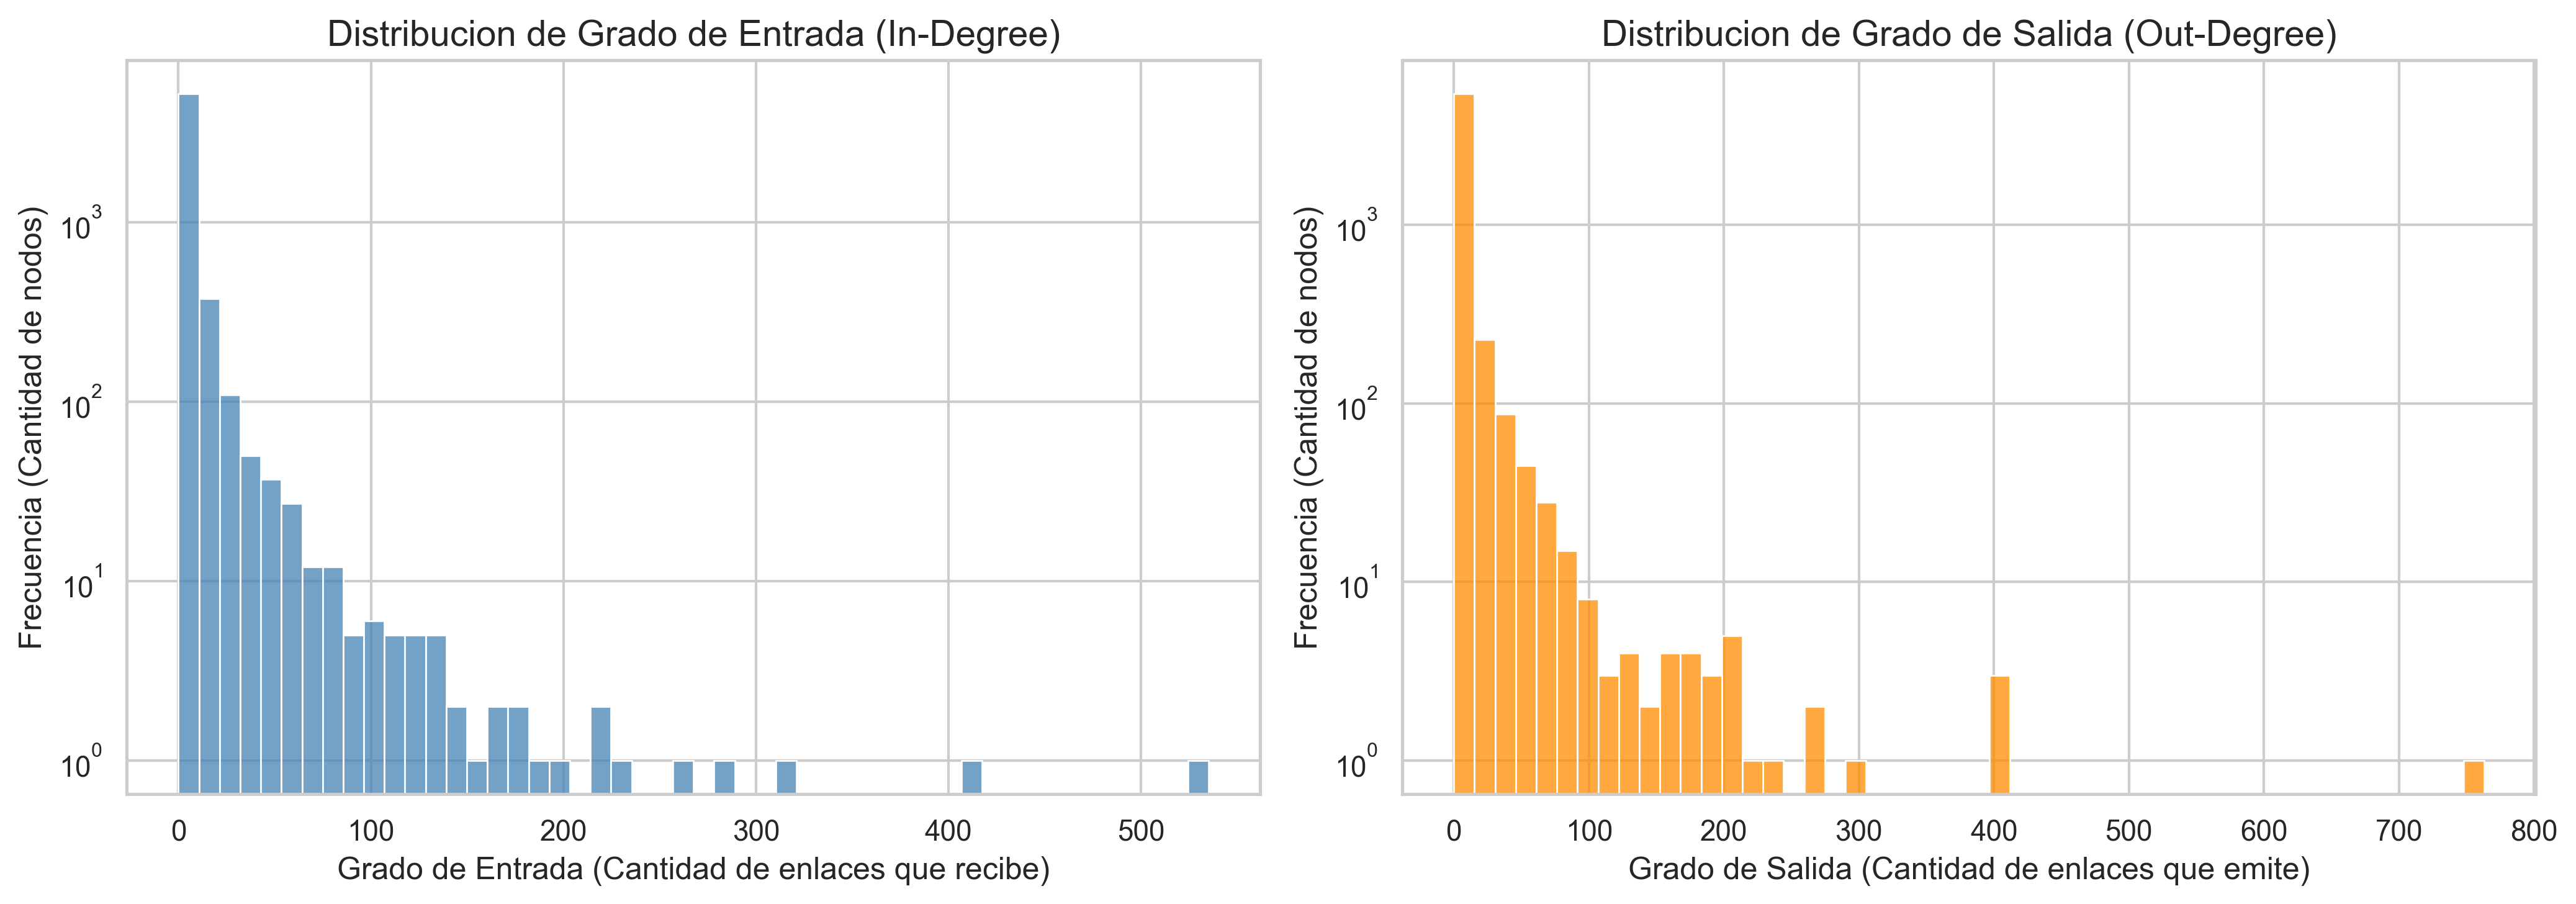
\includegraphics[width=0.8\textwidth]{plots/P3a_distribucion_grados.png}
\end{figure}


\subsubsection*{(b) Nodos colgantes}



\textbf{¿Por qué la presencia de nodos colgantes es problemática para PageRank?}


PageRank modela la navegación por medio de "caminos aleatorios" buscando analizar su convergencia.
en este sentido , si nuestro "Caminante aleatorio" llega a un nodo colgante (sin aristas de salida) se quedara atrapado, luego esto implica que la matriz no converge a nada. Por otro lado, si lo analizamos en términos matriciales, se tiene que la columna asociada a ese nodo en la matriz de hipervínculos $H$ poseerá únicamente 0, y por ende no será estocástica y haciendo que el algoritmo de iteración de potencias pierda probabilidades con cada iteración, impidiendo una convergencia a alguna distribución válida

\textbf{¿Cómo se resuelve con la matriz columna-estocástica $S$?}

La solución para este problema es "Forzar" a que la matriz sea estocástica. Para esto vamos a sustituir la columna llena de 0 por vectores uniformes donde su entrada vale $1/n$ con n como la cantidad total de nodos. Esto significa que cuando nuestro elemento "caminante" llegue al nodo problemático, se teletransporta aleatoriamente a cualquier otro con cualquier otro nodo con igual probabilidad, permitiendo su convergencia y que la nueva matriz S sume a 1



\subsubsection*{(c) Top 10 nodos por grado de entrada y salida}



\begin{figure}[H]
\centering
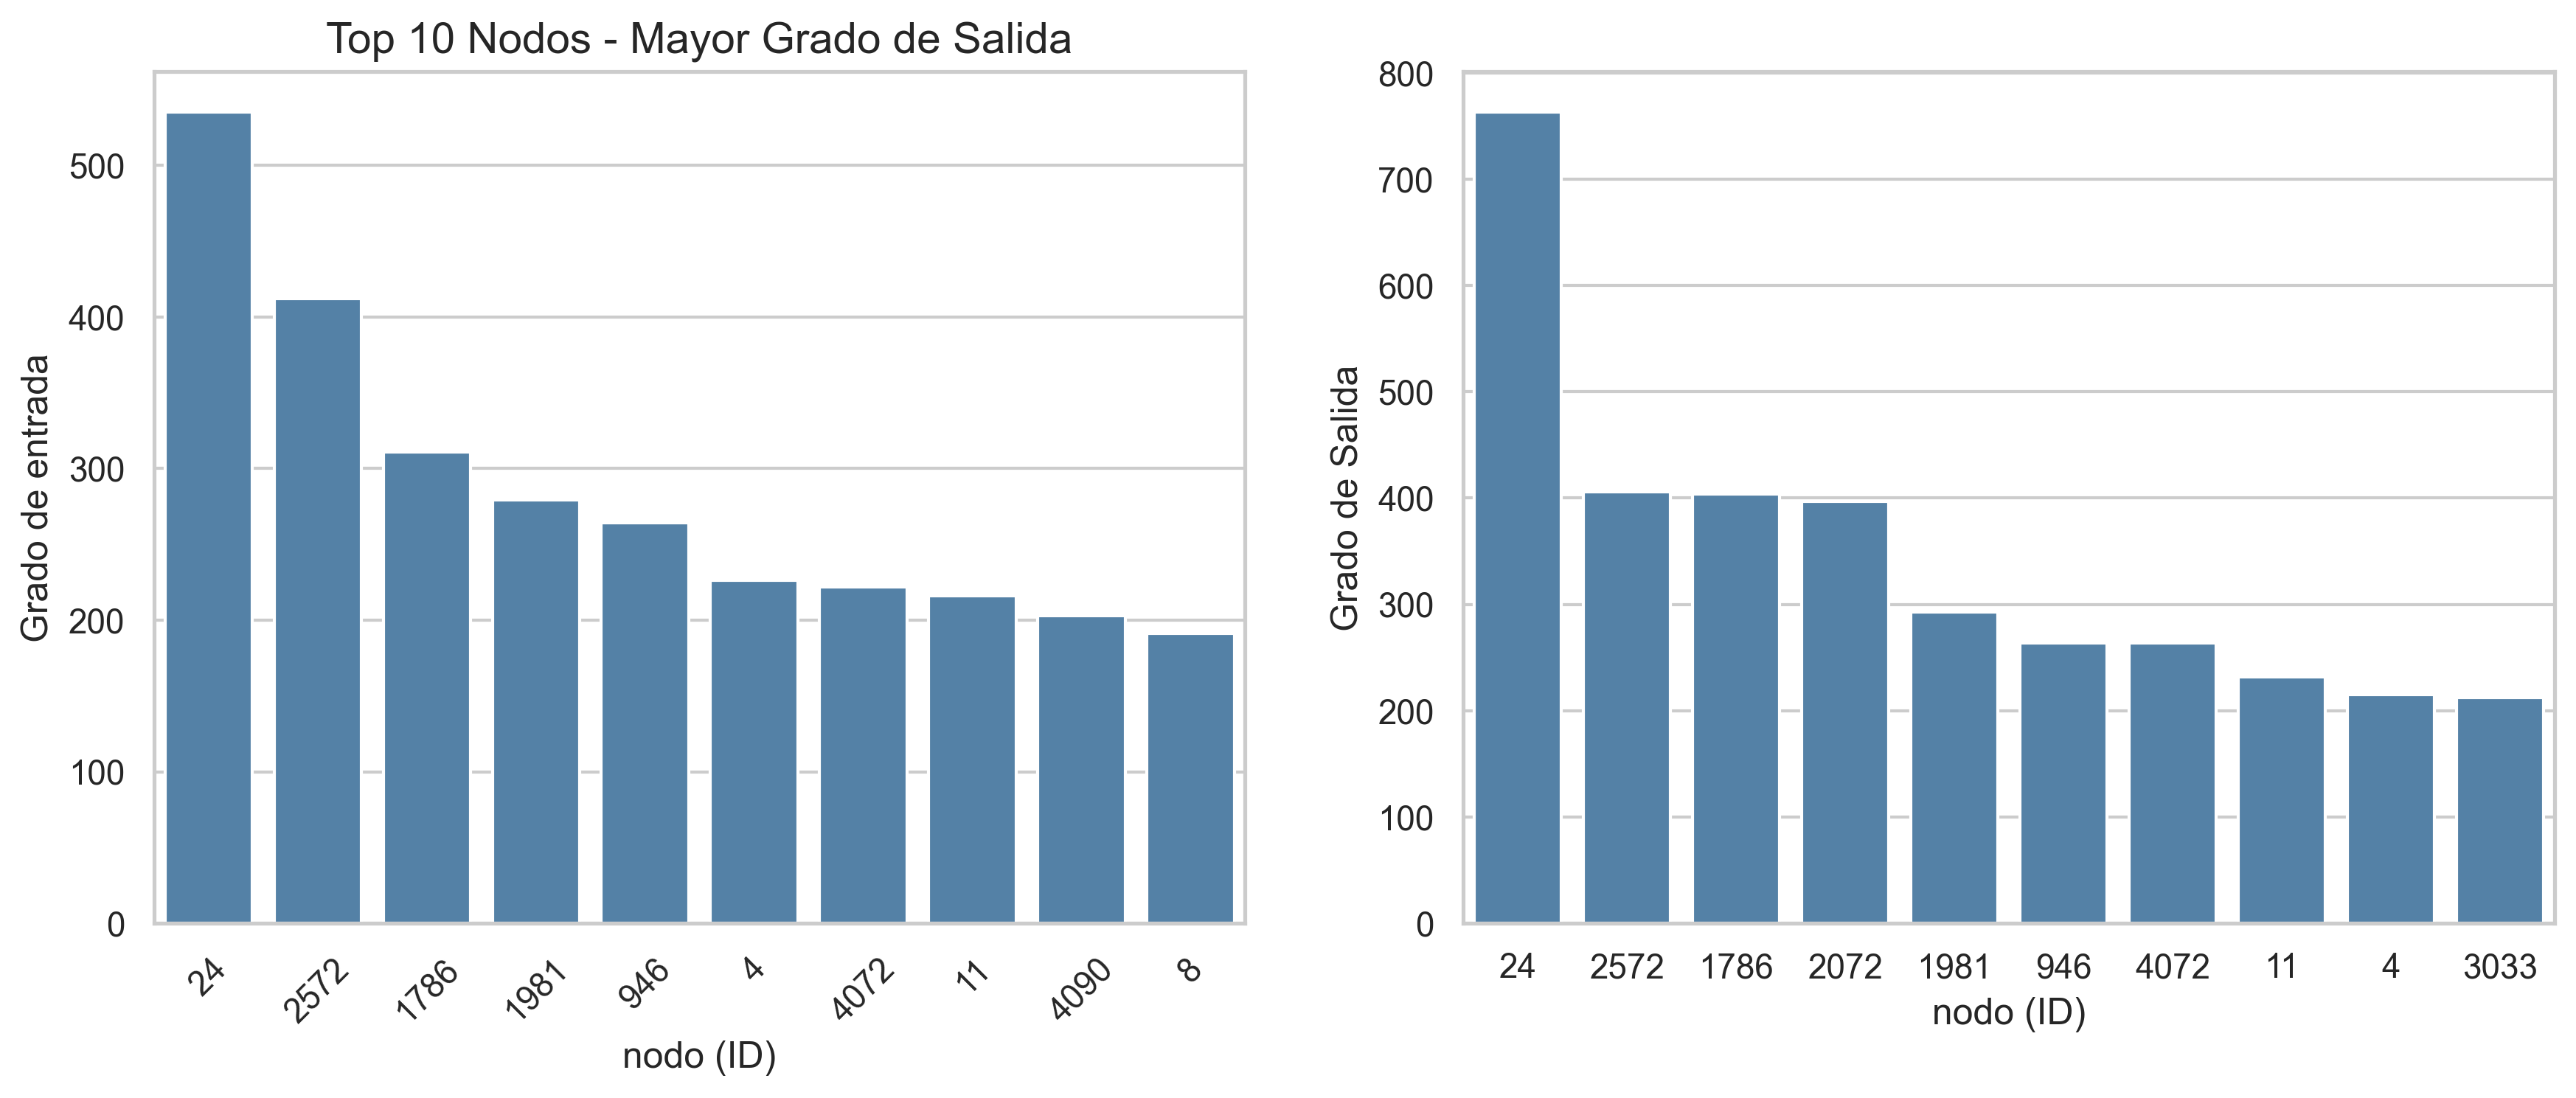
\includegraphics[width=0.8\textwidth]{plots/P3c_grafico.png}
\end{figure}


\subsection*{d ) Analizar conexidad de la red de bitcoin}



Se puede notar que la red no es ni fuertemente conexa ni débilmente conexa, respecto a que la red no sea fuertemente conexa, esto era esperable, puesto que en la vida real es relativamente común que ciertas entidades depositen o hagan mucha transacción con nodos específicos y que esto no suceda en el caso contrario, a sí mismo que la red no sea débilmente conexa se puede explicar con la variabilidad y la forma en la que se hacen las transacciones, para ser débilmente conexa se esperaría que las transacciones se hagan de ambos lados (que 2 nodos se transfieran dinero de forma constante) cosa que no es esperable en la vida real



\subsection*{P4: Construcción de la Matriz de Google}


\subsubsection*{(a) Matriz de hipervínculos $H$}



\subsubsection*{(b) Matriz columna-estocástica $S$}



poodemos notar que el margen de error encontrado se corresponde con errores asociados al computo de numeros de coma flotante, y por tanto son validos con nuestros calculos



\subsubsection*{(c) Matriz de Google $G$}



Nosotros usamos: 
$\alpha = 0.85$ el cual es el estandar de la industria puesto que este valor equilibria la influencia de la estructura del grafo con el salto aleatorio $1 - \alpha$ que garantiza una convergerncia rapida sin depender de la forma especifica del grafo.
Esto ademas basandonos en el siguiente [estudio](https://archive.org/details/google-pagerank-algorithm-using-efficient-damping-factor/mode/1up)
Por otro lado, las entradas deben de ser siempre positivas en nuestra matriz de Google, este puesto que si no nuestra matriz podría tener nodos que reciben un input sin liberar ningún output, cosa que tanto impediría la utilidad de la misma en ciertos contextos, y además, haría que la convergencia dependa del punto inicial de partida. Esto mismo no nos es útil, puesto que buscamos encontrar que nuestra matriz converja para cualquier punto $x_0$ elegido




\subsection*{P5: Cálculo del PageRank mediante Iteración de Potencias}



\subsubsection*{P5(a): Iteración de potencias}

Partimos del vector uniforme $\mathbf{r}^{(0)} = \mathbf{1}/n$ e iteramos

$$\\mathbf{r}^{(k+1)} = G\\,\\mathbf{r}^{(k)}$$

hasta que $\|\mathbf{r}^{(k+1)} - \mathbf{r}^{(k)}\|_1 < \varepsilon = 10^{-10}$.



\subsubsection*{P5(b): Curva de convergencia}

Graficamos $\|\mathbf{r}^{(k+1)} - \mathbf{r}^{(k)}\|_1$ en escala logarítmica.  



\begin{figure}[H]
\centering
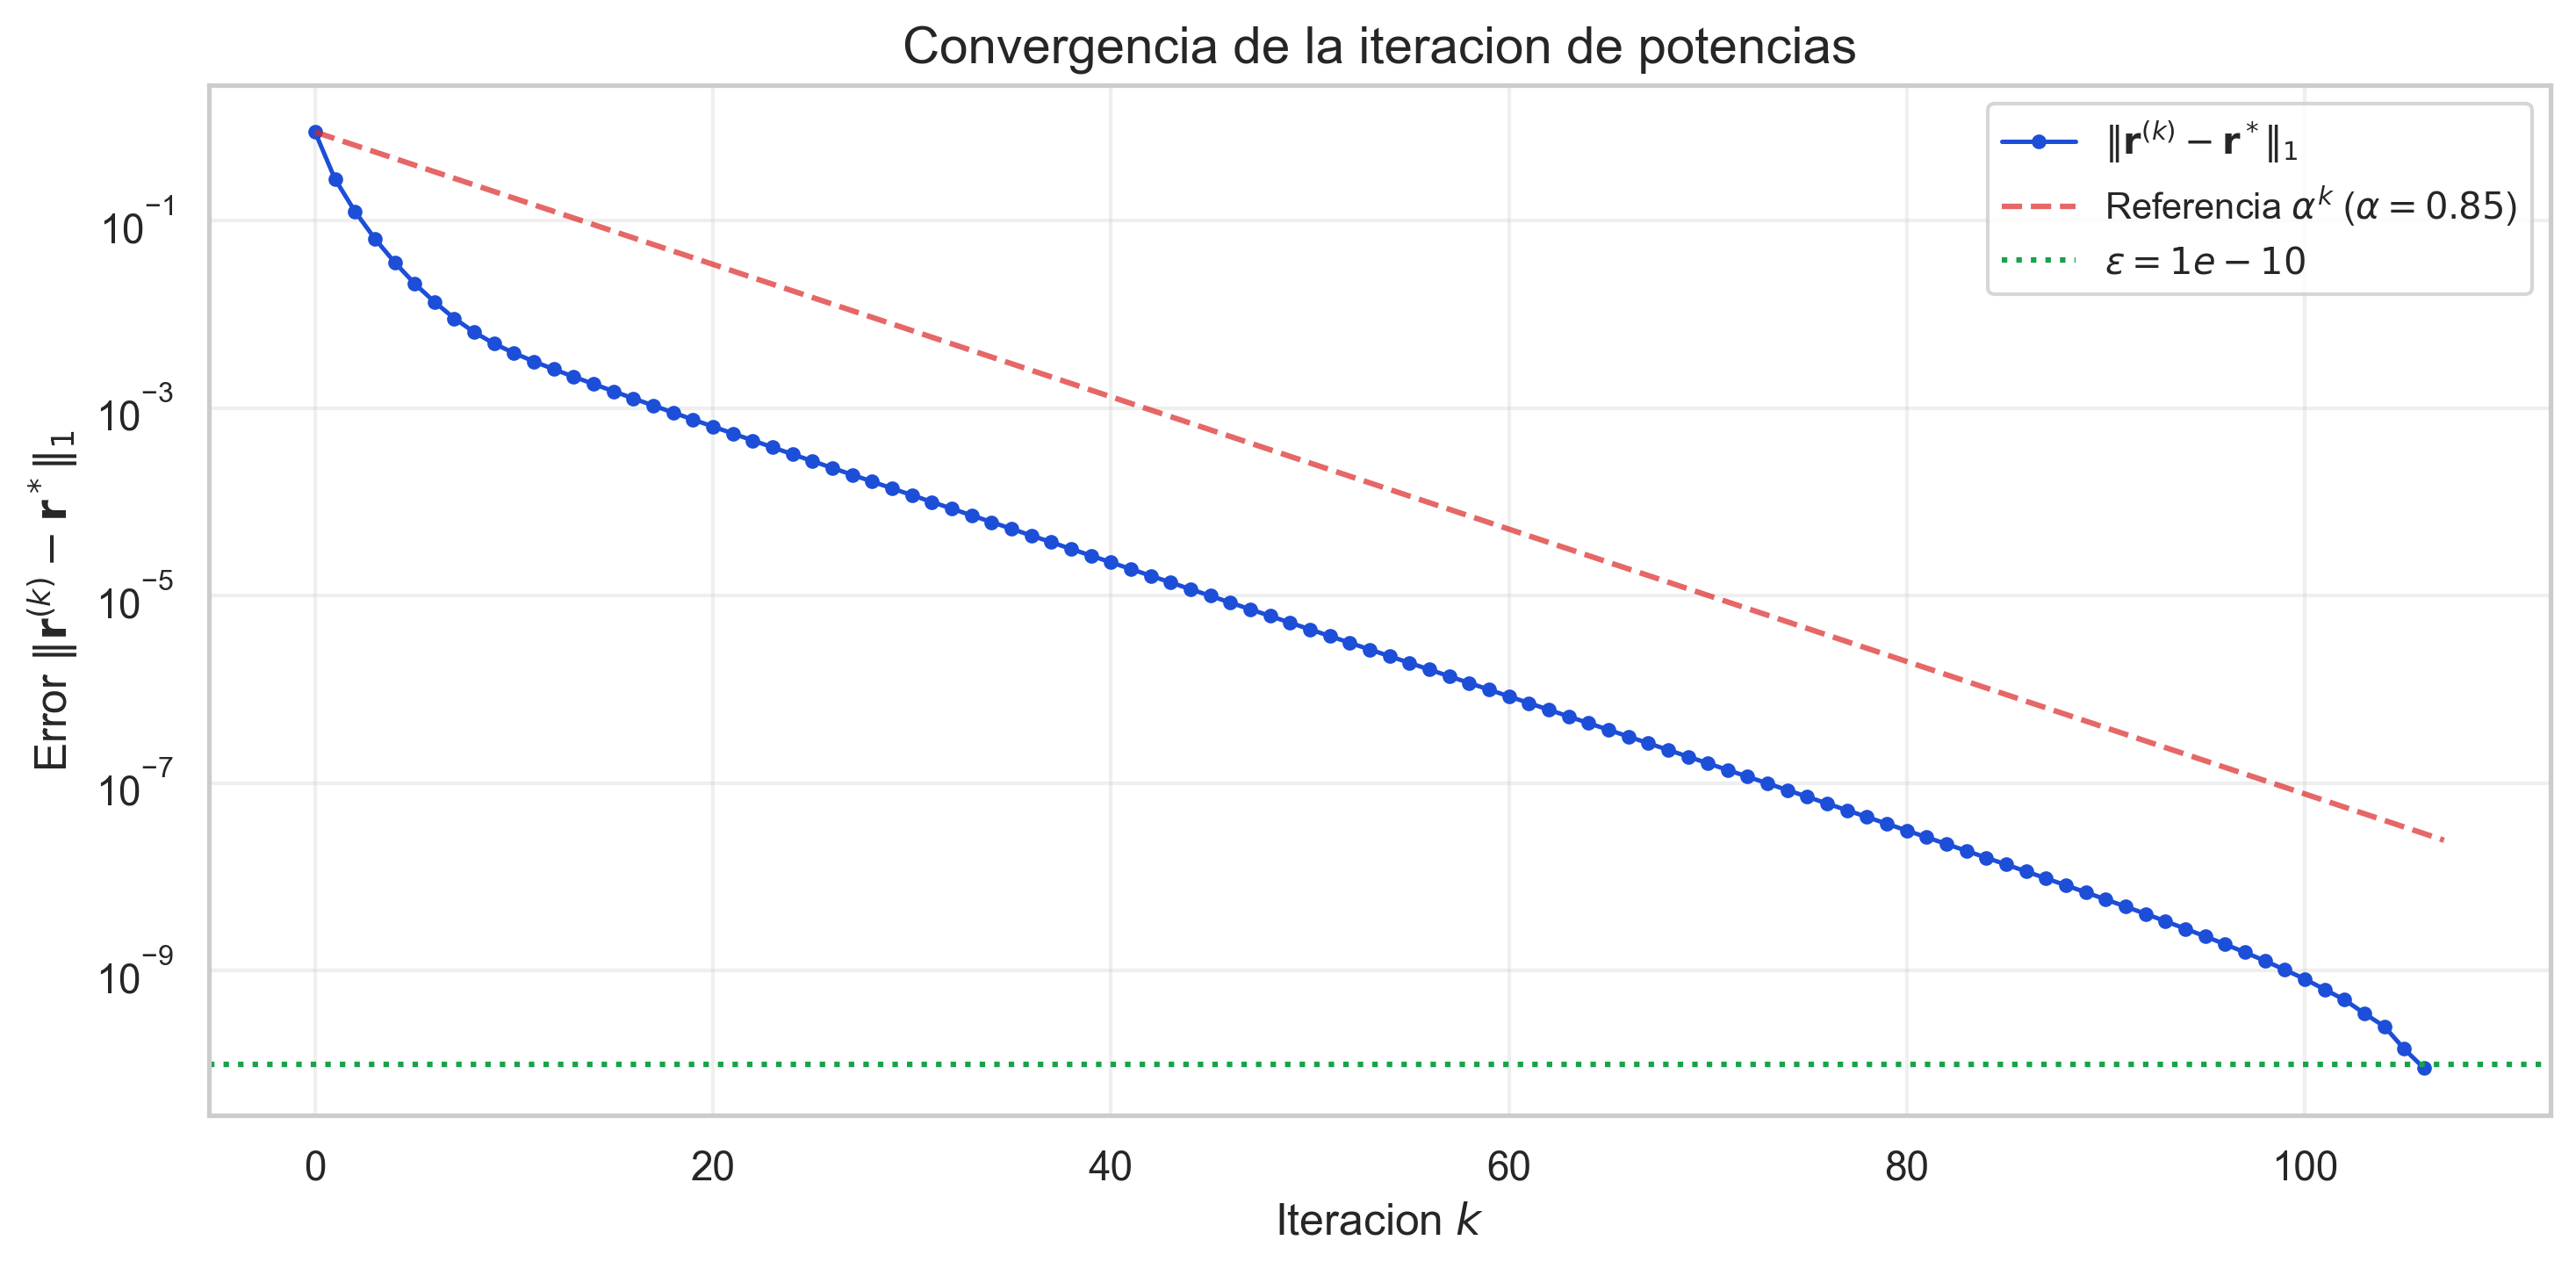
\includegraphics[width=0.8\textwidth]{plots/P5b_grafico.png}
\end{figure}


El decaimiento es geometrico con razon $\approx \alpha = 0.85$ en la zona central del grafico (linea recta en escala log), confirmando la teoria.  
La curvatura al final se debe a que usamos como $\mathbf{r}^*$ la ultima iteracion computada y no el vector estacionario exacto: 
cuando $\mathbf{r}^{(k)}$ se acerca a $\mathbf{r}^{(k_{\text{final}})}$, la distancia colapsa artificialmente a cero por aritmetica de punto flotante.



\subsubsection*{P5(c): Verificación de propiedades del vector estacionario}

El teorema de Perron-Frobenius garantiza que, para una matriz, como la de Google $G$, columna-estocástica (columnas suman 1), irreducible (todas las entradas son > 0 por la teletransportación) y aperiódica (diagonal > 0):

1. Existe un único vector propio $\mathbf{r}^*$ asociado al valor propio dominante $\lambda_1 = 1$.
2. Todas las componentes de $\mathbf{r}^*$ son estrictamente positivas: $r_i^* > 0 \; \forall i$.
3. Al normalizar $\|\mathbf{r}^*\|_1 = 1$, el vector representa una distribución de probabilidad (la distribución estacionaria del navegante aleatorio).

La irreducibilidad se asegura porque $G$ tiene todas sus entradas positivas (gracias al término de teletransportación $(1-\alpha)/n$), y una matriz con todas las entradas positivas es irreducible y aperiódica.



\subsubsection*{P5(d): Top 20 nodos por PageRank}



Dado que Bitcoin OTC es una plataforma de transacciones anónimas el datatset no incluía más que un número entero positivo para identificar cada nodo, ningún metadato.



\subsection*{P6: PageRank vs. Grado de Entrada}



\subsubsection*{P6(a): Gráfico disperso y correlación de Pearson}




\begin{figure}[H]
\centering
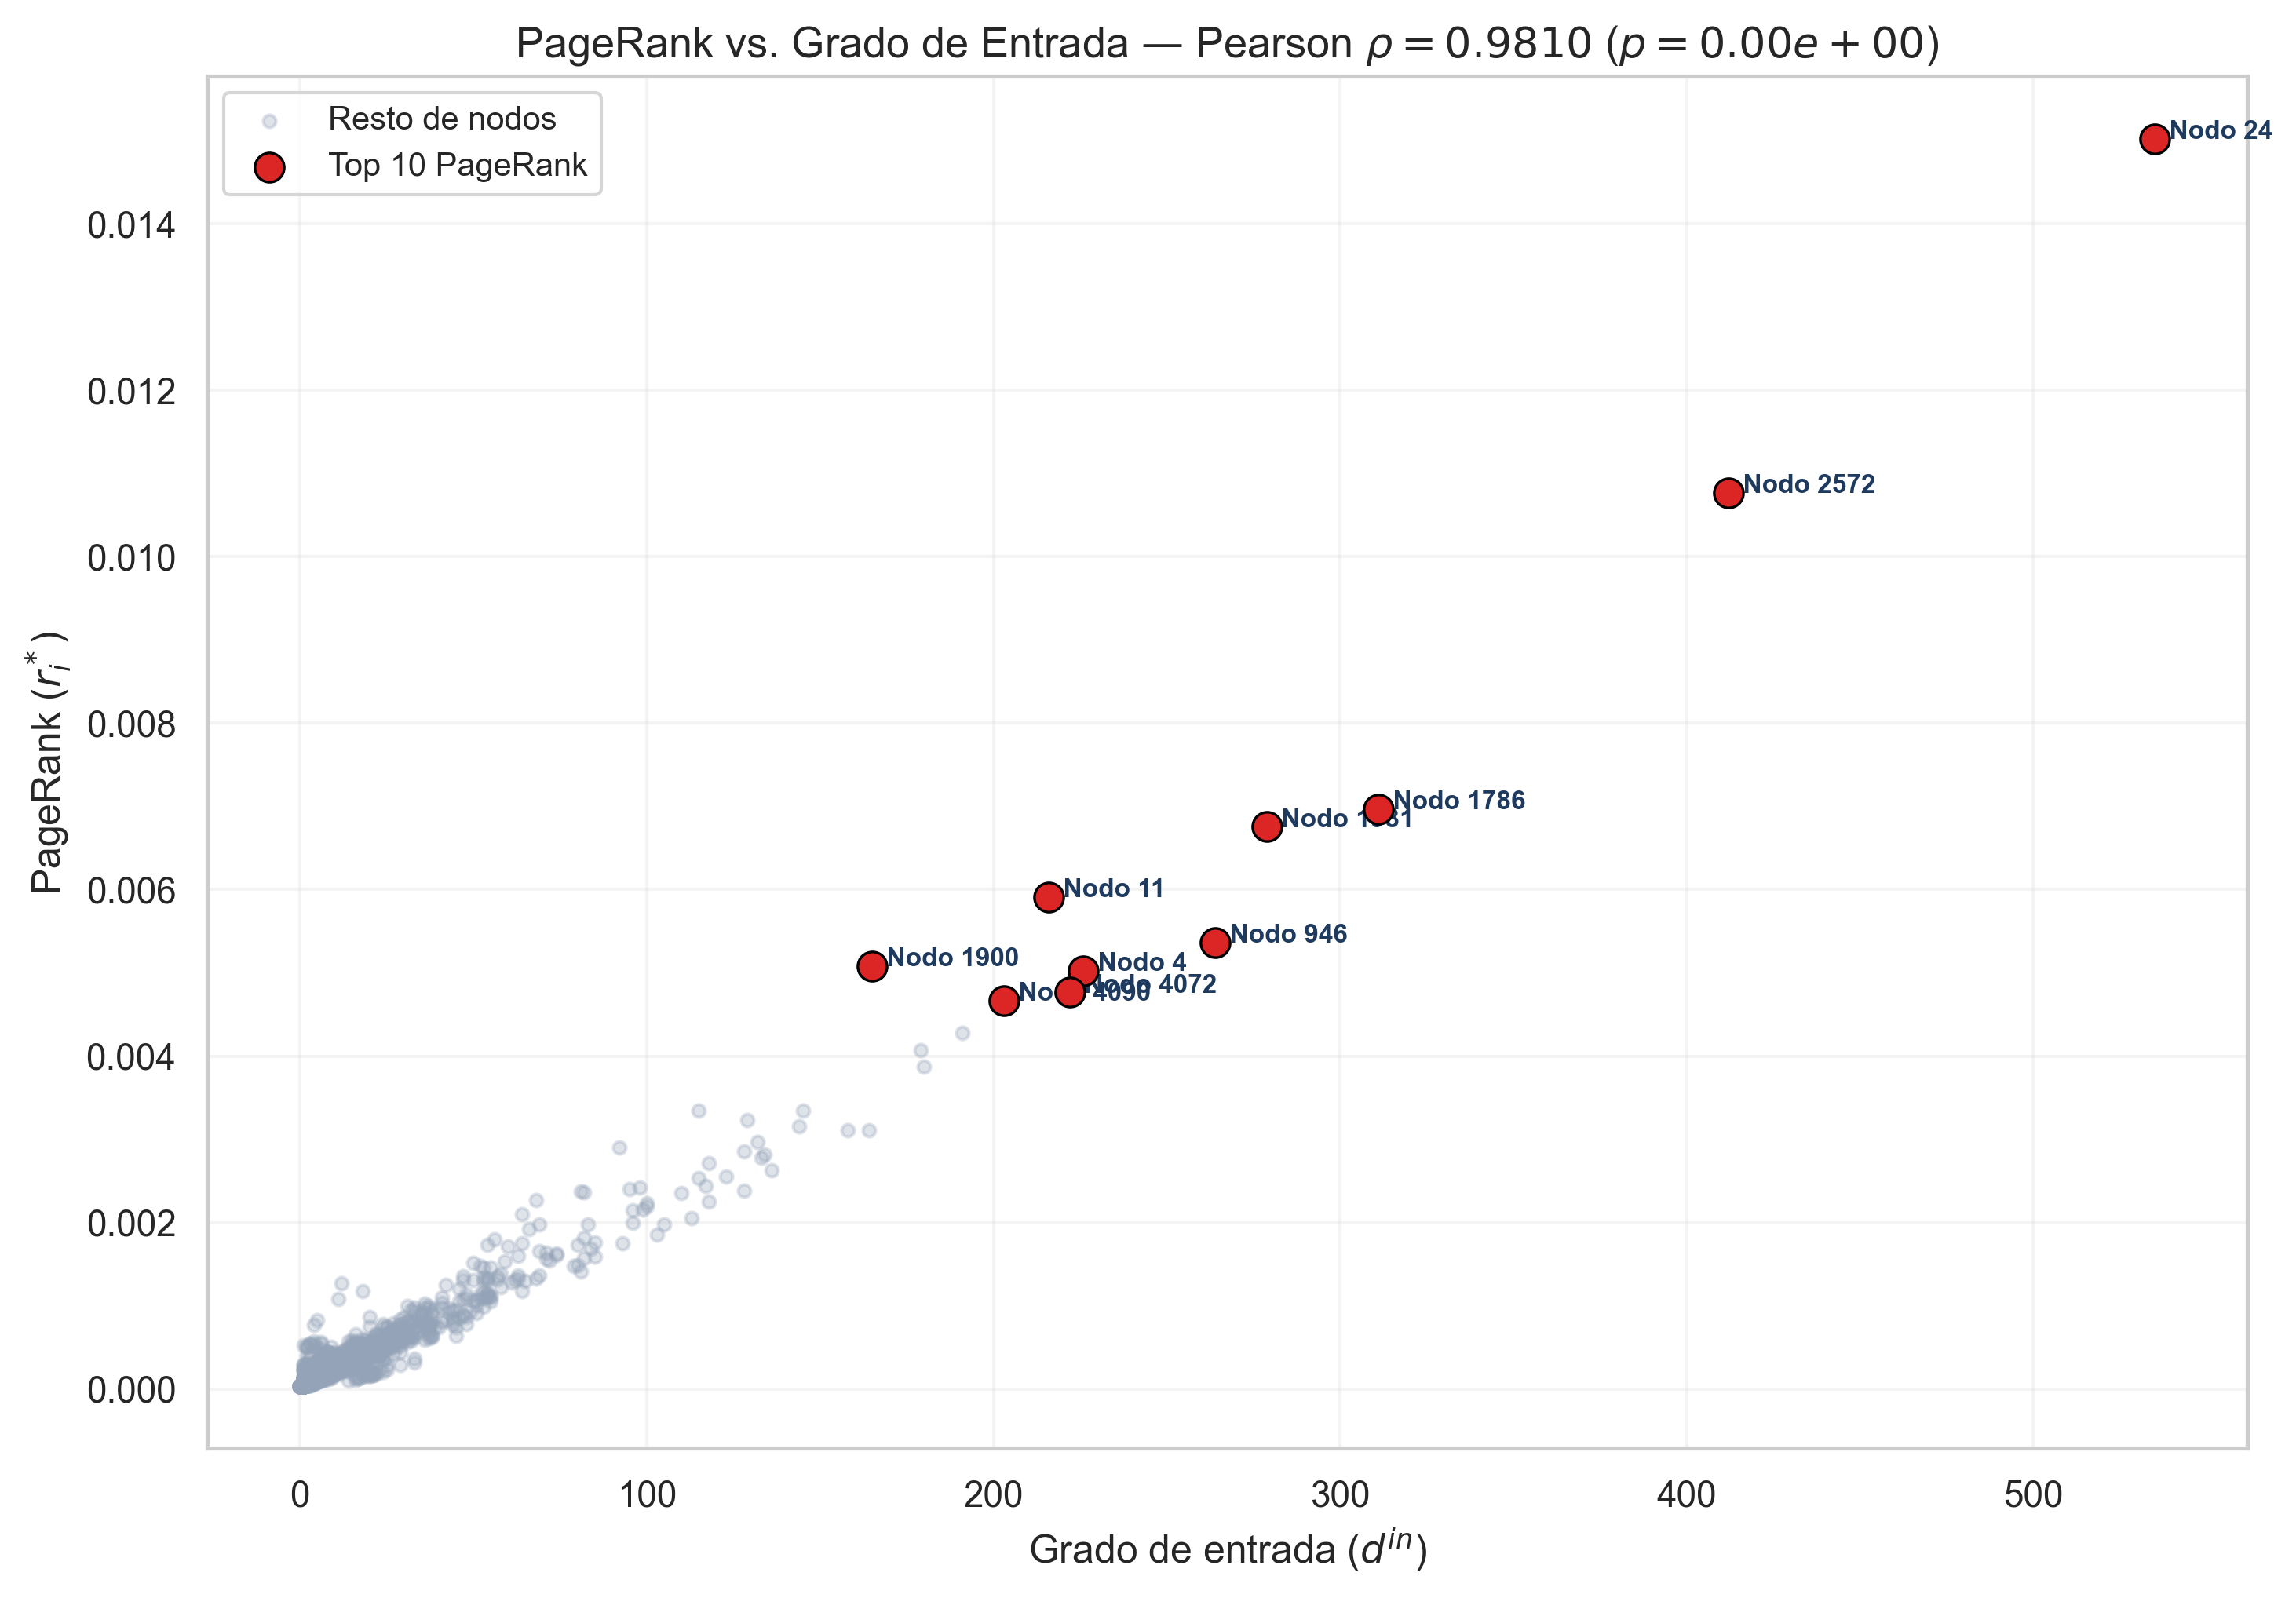
\includegraphics[width=0.8\textwidth]{plots/P6_correlacion_pearson.png}
\end{figure}


\subsubsection*{P6(b): Nodos donde PageRank y grado de entrada difieren}



- \textbf{CASO 1:} Los nodos \textbf{2496} y \textbf{1030} tienen grados de entrada aceptables (12 y 11 conexiones). Sin embargo, PageRank dispara su valoración jerárquica (Score PR ~53-59). Esto indica que gozan de la confianza de la élite de la red; reciben pocas calificaciones, pero muy valiosas.
- \textbf{CASO 2:} Los nodos \textbf{4556} o el \textbf{4546} lograron acumular bastantes enlaces (33 y 24) (Score $d^{in}$ ~20-28). No obstante, PageRank los castiga (Score PR ~8-14) porque sus conexiones probablemente provienen en su mayoría de usuarios periféricos o recién llegados. Inflaron sus números, pero carecen de influencia real en Bitcoin OTC.



\subsubsection*{¿Por qué se uso `method='dense'` (Dense Ranking)?}



\begin{figure}[H]
\centering
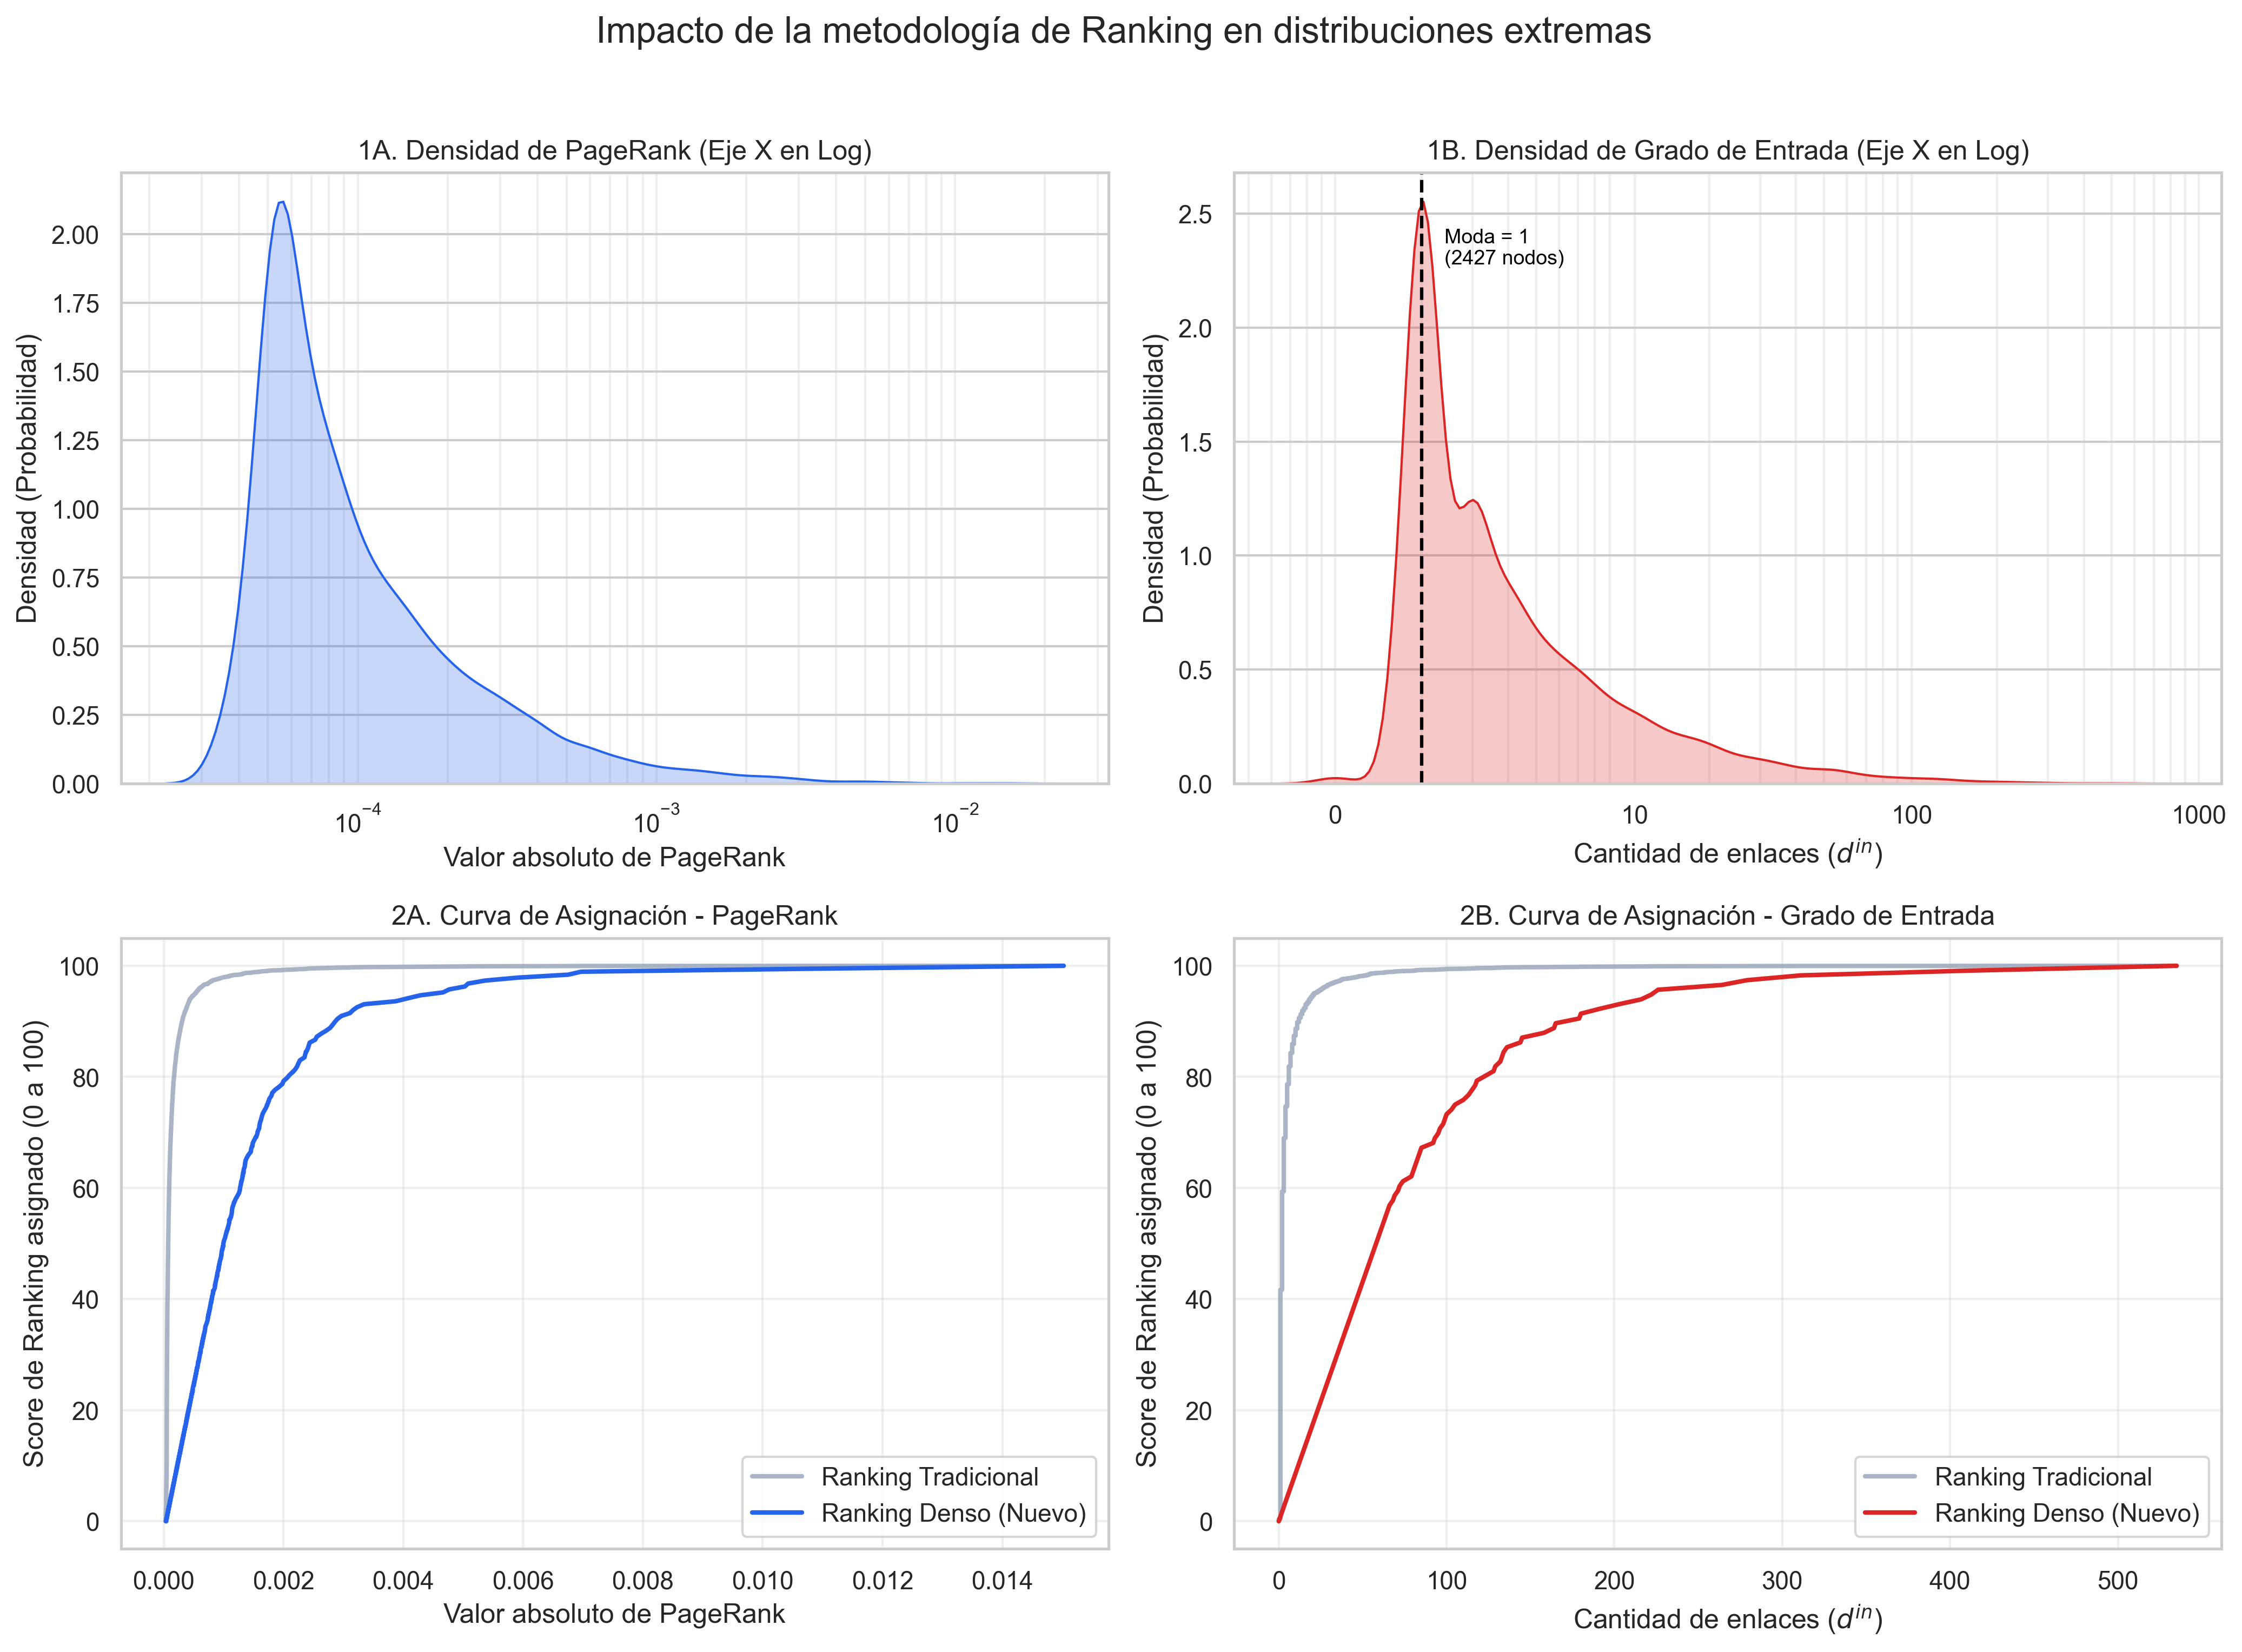
\includegraphics[width=0.8\textwidth]{plots/P6_KDE_y_curvas_asignacion.png}
\end{figure}


Los gráficos revelan una desigualdad notable en la red. Los gráficos de densidad (KDE) muestran una acumulación gigantesca en valores mínimos; la mayor concentración de la red está exactamente en $d^{in} = 1$, agrupando a 2427 nodos (41.3\% de los usuarios). 

Esta asimetría invalida la comparación directa, ya que la mayoría de la red colapsaría a un puntaje de `0`.

\textbf{El Problema del Ranking Tradicional}  
Para evidenciar esto, definimos un Score Tradicional (0 a 100) calculado linealmente según la posición absoluta del nodo (donde el 1° lugar absoluto = 100, y el lugar 5881 = 0). 

Como se aprecia en las Curvas de Asignación (Fila 2), este método no es óptimo para $d^{in}$ (gráfico 2B). La línea gris dibuja "acantilados" completamente verticales: al haber 2427 nodos empatados en $d^{in} = 1$, el sistema los ordena por posiciones arbitrarias continuas, haciendo que su score se desplome desde ~40 hasta casi 0.

\textbf{La Solución: Ranking Denso (Nuevo Score)}
Para hacer ambas métricas estadísticamente comparables, aplicamos un ranking `dense` (curvas a color en la fila 2). Este método ignora el volumen de empates y asigna un "Nivel" único a cada valor en la red. 

\textit{(Ejemplo con 7 datos fuertemente sesgados: `[500, 2, 1, 1, 1, 0, 0]`)}
- \textbf{Score Tradicional (0-100 por posición):} Se calcula linealmente usando la posición absoluta del 1° al 7° lugar. Los puntajes quedarían así:
  - El `500` recibe \textbf{100.0}
  - El `2` recibe \textbf{83.3}
  - Los tres `1` reciben \textbf{66.7}, \textbf{50.0} y \textbf{33.3} respectivamente (una caída vertical para exactamente el mismo valor).
  - Los dos `0` reciben \textbf{16.7} y \textbf{0.0}.

- \textbf{Score Denso (0-100 por niveles únicos):} Existen solo 4 valores únicos en la red, por lo que se crean 4 escalones equitativos:
  - El `500` recibe \textbf{100.0}
  - El `2` recibe \textbf{66.7}
  - \textbf{Todos} los `1` reciben exactamente el mismo score de \textbf{33.3}.
  - \textbf{Todos} los `0` reciben exactamente el mismo score de \textbf{0.0}.


Aplicamos esta misma lógica a ambas métricas:
- \textbf{Para el Grado de Entrada:} Garantiza que los 2427 nodos con $d^{in} = 1$ reciban exactamente el mismo Score Denso (la línea escalonada roja en 2B).
- \textbf{Para PageRank:} Al ser una variable flotante, PageRank carece de empates naturales; micro-diferencias irrelevantes de $10^{-7}$ separarían nodos por cientos de posiciones (la violenta caída gris al final del gráfico 2A). Para solucionarlo, redondeamos PageRank a 5 decimales. Esto filtra el ruido y crea niveles de densidad artificiales parecidos a los de $d^{in}$, estabilizando más la curva (línea azul en 2A).

Al escalar estos "Niveles Densos" de 0 a 100, evaluamos equitativamente qué peldaño ocupa realmente cada nodo sin las deformaciones de los empates masivos.






\subsection*{P7: Interpretación de resultados}

En esta seccion buscamos interpretar la Page rank calculada en el contexto de Bitcoin. En este sentido debemos mencionar, que nuestra red es es \textit{firmada}(ratings de -10 a + 10) pero al momento de construir $H$ nosotros unicamente usamos la existencia de esta arista $j \to i$ , no su signo, es decir, que nuestra page rank calculada da un "voto" a un nodo por cada que alguien lo califica, sea con ujna calificacion posiutiva op negativa, luego antes de decir "los nodos con mayor page rank son los mas confiable" . nos es de utilidad revisar el signo de sus calificaciones, esto puesto que un page rank alto puede significar tanto un usuario con calificaciones excelentes como uno muy denunciado o polemico



\subsubsection*{a) Nodos con mayor Pagerank e interpretacion del dominio}

Para interpretar en este sentido el ranking, vamos a alimentar nuestro Pagerak con el rating promedio percivido de cada nodo (El promedio de sus aristas entradas) justo con la fraccion de calificaciones negativas, buscando crear un top-page rank entre usuarios con reputaciones consolidadas y filtrando a los usuarios que son "Importante" por sus conexiones negativas entre los demas



\textbf{Interpretaciones:}

Podemos notar que ningún nodo de nuestro top 20 presenta un grado de ser "sospechoso" , todos presentan un `rating\_prom\_recibido` positivo de entre 0.61 a 3.54 en la escala de -10 a 10 y una `fraccion\_negativas\_recibidos` baja de entre 0\% a un 16\% estos nos dice:

Estos nodos son un hub de actividad. En especial en nodo 24 el cual lidera con diferencia ($d_{in} = 535$ , $d_{out} = 763$) esto se entiende como alguien con mucho tiempo operando, y que califica y es calificado de forma masiva, con reputaciones positivas, hay otro caso como el 4(rating de 3.54) o el 11 (rating de 2.84) que poseen menos volumen, pero un mejor promedio, en general podemos notar que el top 20 son usuarios con cientos de calificaciones. La mayoría buenas.

Podemos notar entonces que el algoritmo no busca premiar a quienes reciben más calificaciones en bruto, sino que a quien es respaldado por la comunidad, de esta forma este grupo resulto que es el núcleo de traders confiables. Esto contrasta con nuestra hipótesis inicial de: EL pageRank estándar no está aislando a los actores de Desconfianza, sino que está identificado y uniendo a los usuarios más respaldados de la plataforma



\subsection*{b): Sub grafo inducido con los nodos de mayor PageRank}



Visualizaremos el sub grafo inducido por los 40 nodos de mayor PageRank. En este sentido nosotros no poseemos de atributos categóricos naturales(usuarios anónimos, id ,entre otros) es por esto que usaremos como atributo para unir los nodos el rating de confianza construido anteriormente, de forma que los nodos en verdes serán confiables, y los nodos en rojos eran los sospechosos / Denunciables.



\begin{figure}[H]
\centering
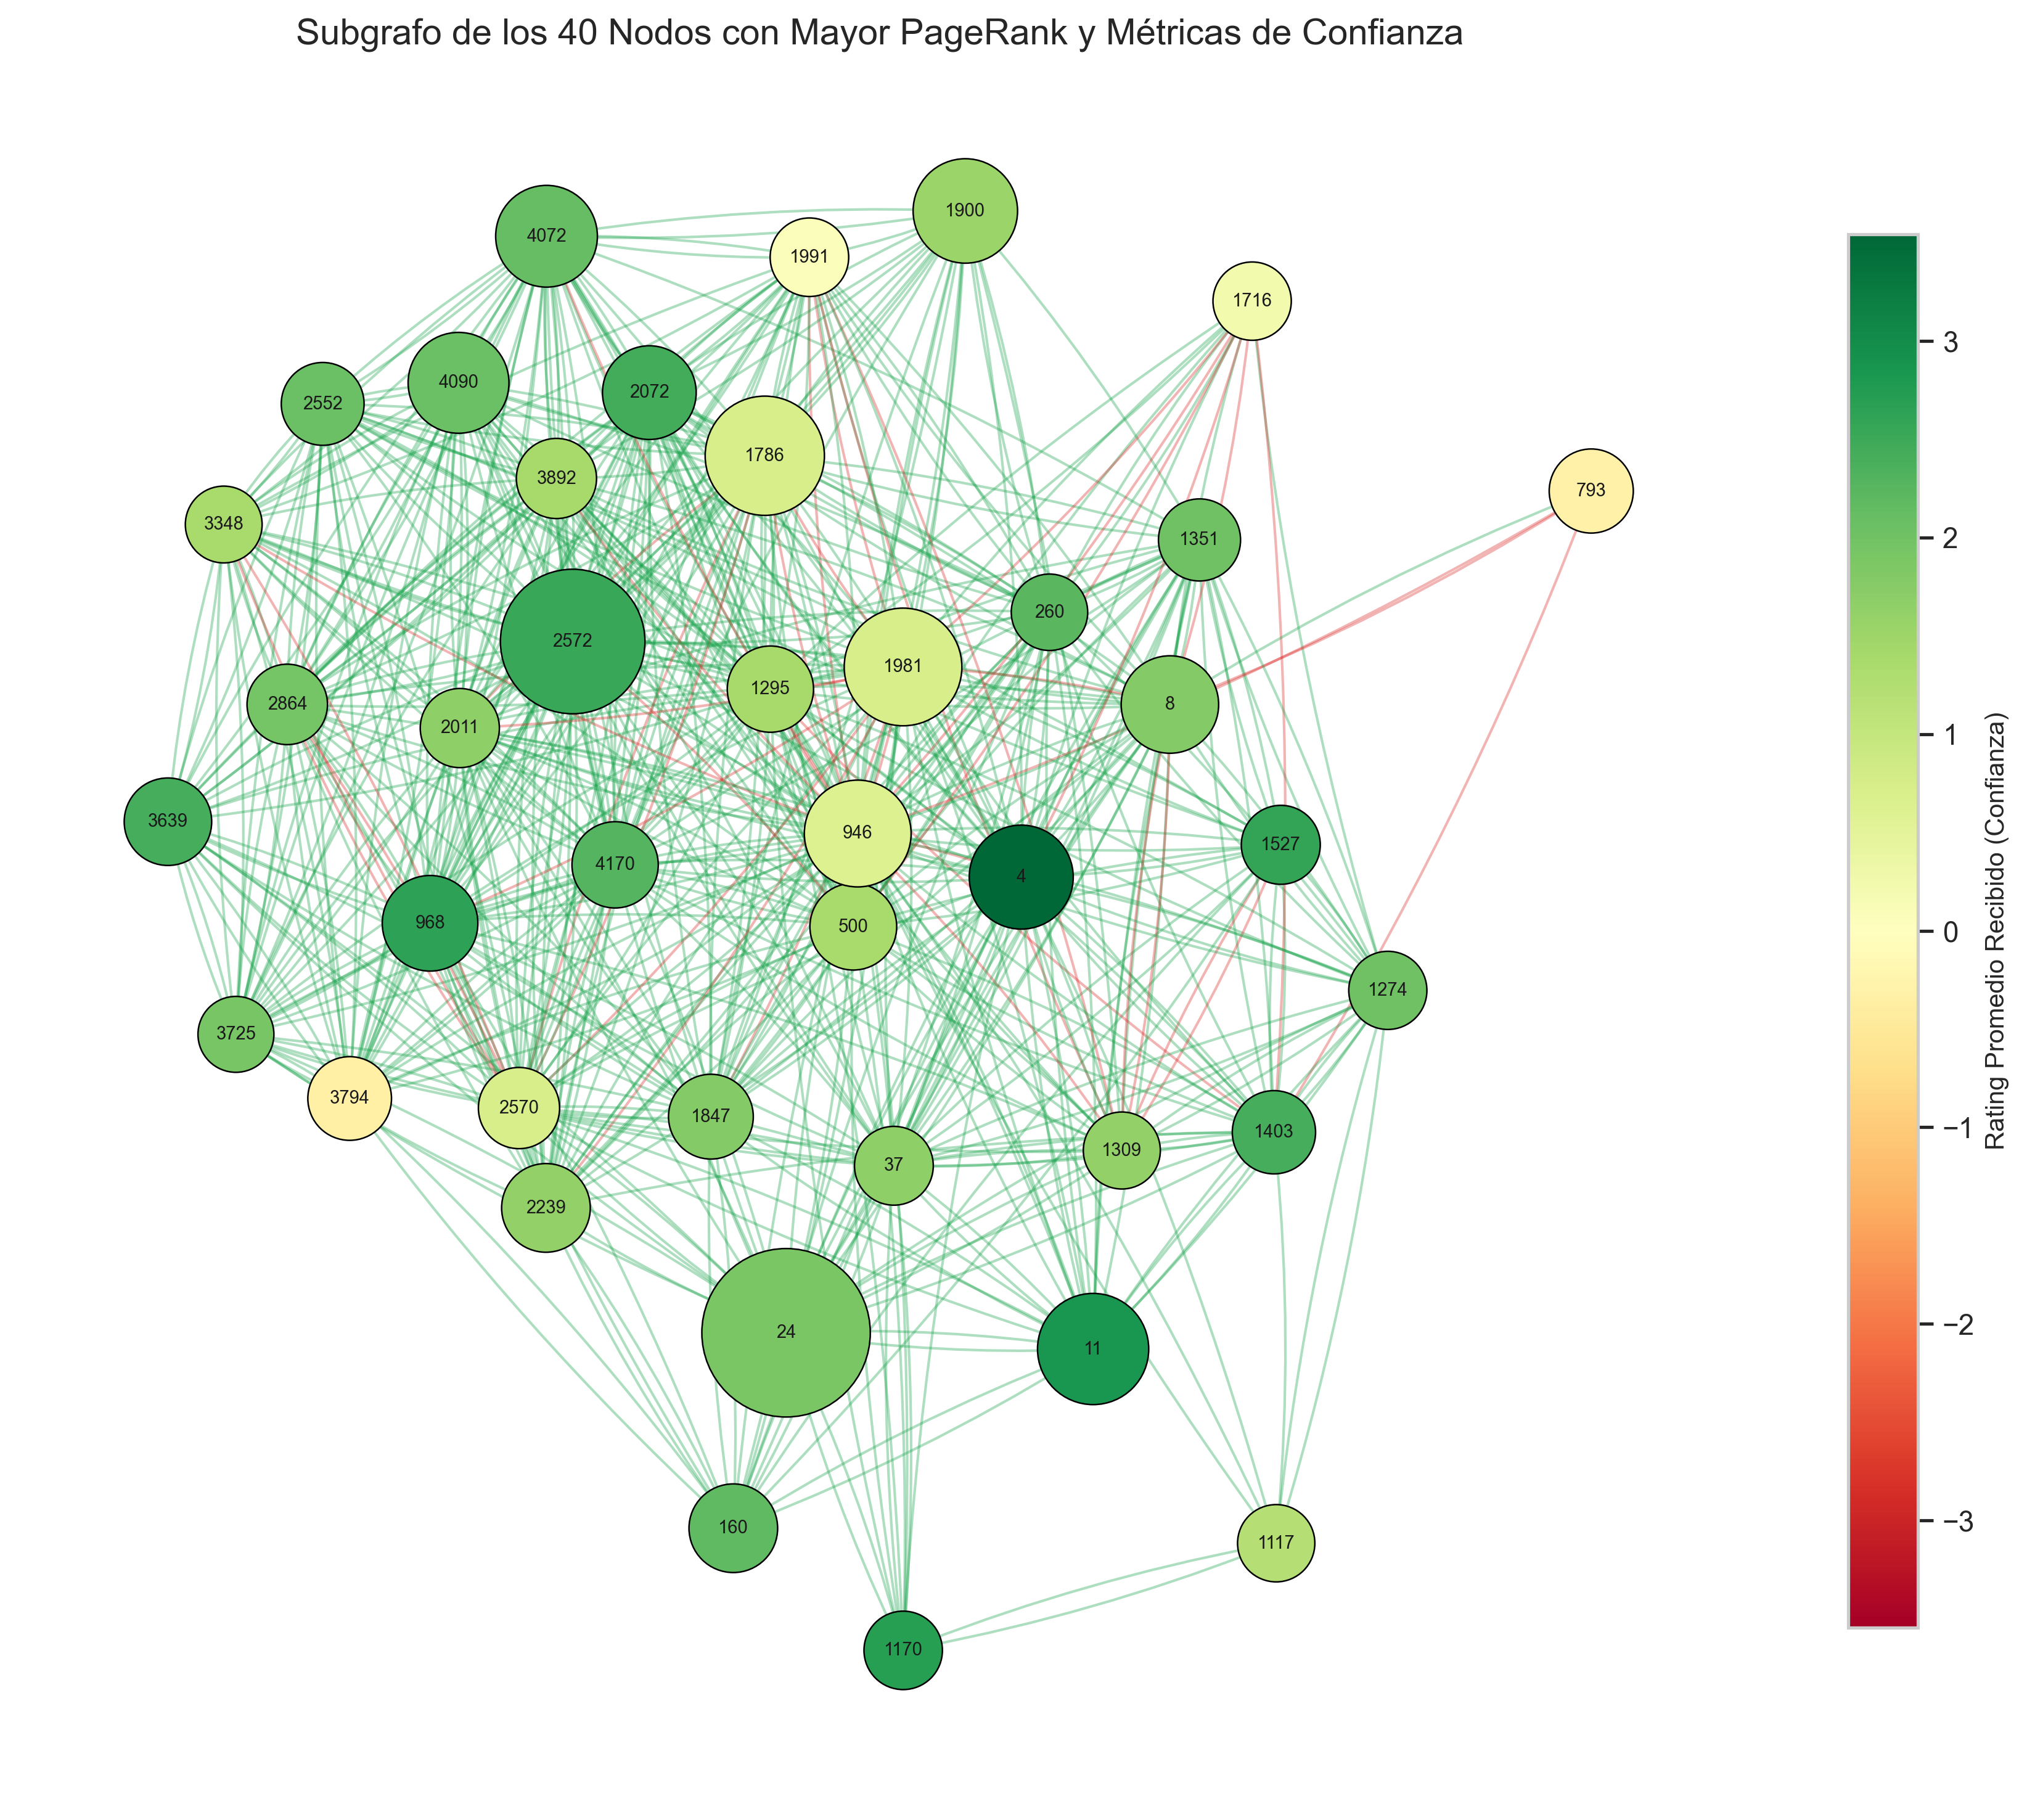
\includegraphics[width=0.8\textwidth]{plots/P7b_grafico.png}
\end{figure}


\textbf{Comentario de estructura observada}

Podemos notar que tenemos una estructura densa, similar a un "clúster" donde tenemos gran parte de los nodos interconectados entre sí, esto es consistente con lo que se vio anteriormente, un cúmulo de traders confiados conectados y que se califican simultáneamente.

Podemos notar además que como tal no existe ningún "nodo rojo". Hay nodos que reciben calificaciones negativas de otras, y nodos que se encuentran entre medio de una calificación positiva y negativa. Estos es consistente con lo visto anteriormente, no tenemos ningún "clúster de desconfianzas", todo Nuestro TOP-40 pertenece al mismo bloque de usuarios bien evaluados.

Además como nodo central tenemos al nodo 24, cosa coherente con los resultados anteriores , de igual forma los 4 y 11 son los que poseen un verde más oscuro, representando siu calidad, pero son notablemente más chicos (cosa ya vista en la tabla de resultados)

Tenemos además 4 nodos principales periféricos que están menos conectados, estos nodos parecen ser nodos que se "colaron" al top 40 sin estar integrados a la comunidad, se puede ver en general que están conectados a nodos de gran confianza o centrales.

Además , se puede notar una clara mayoría en las aristas positivas, en relación con las rojas que representan una mala calificación.





\subsection*{C )¿Los nodos de mayor PageRank pertenecen a un grupo particular?}

Nuestro grafo no posee ninguna tributo de nodo natural, únicamente id, es por esto que para responder nuestra pregunta usaremos como "grupo" la categoría de confianza derivada del rating de promedio recibido creado anteriormente, usando el rango confiable, neutral y sospechoso.

Adicionalmente verificaremos nuestra hipótesis , viendo si los nodos forman un clúster de confianza, midiendo tres predicciones concretas:

1. Densidad interna del sub grafo top-PageRank mayor a la densidad global.
2. Coeficiente de clustering local promedio del top mayor al promedio global.
3. Pesos promedio de aristas dentro del clúster más positivo que los de aristas mixtas.



\begin{figure}[H]
\centering
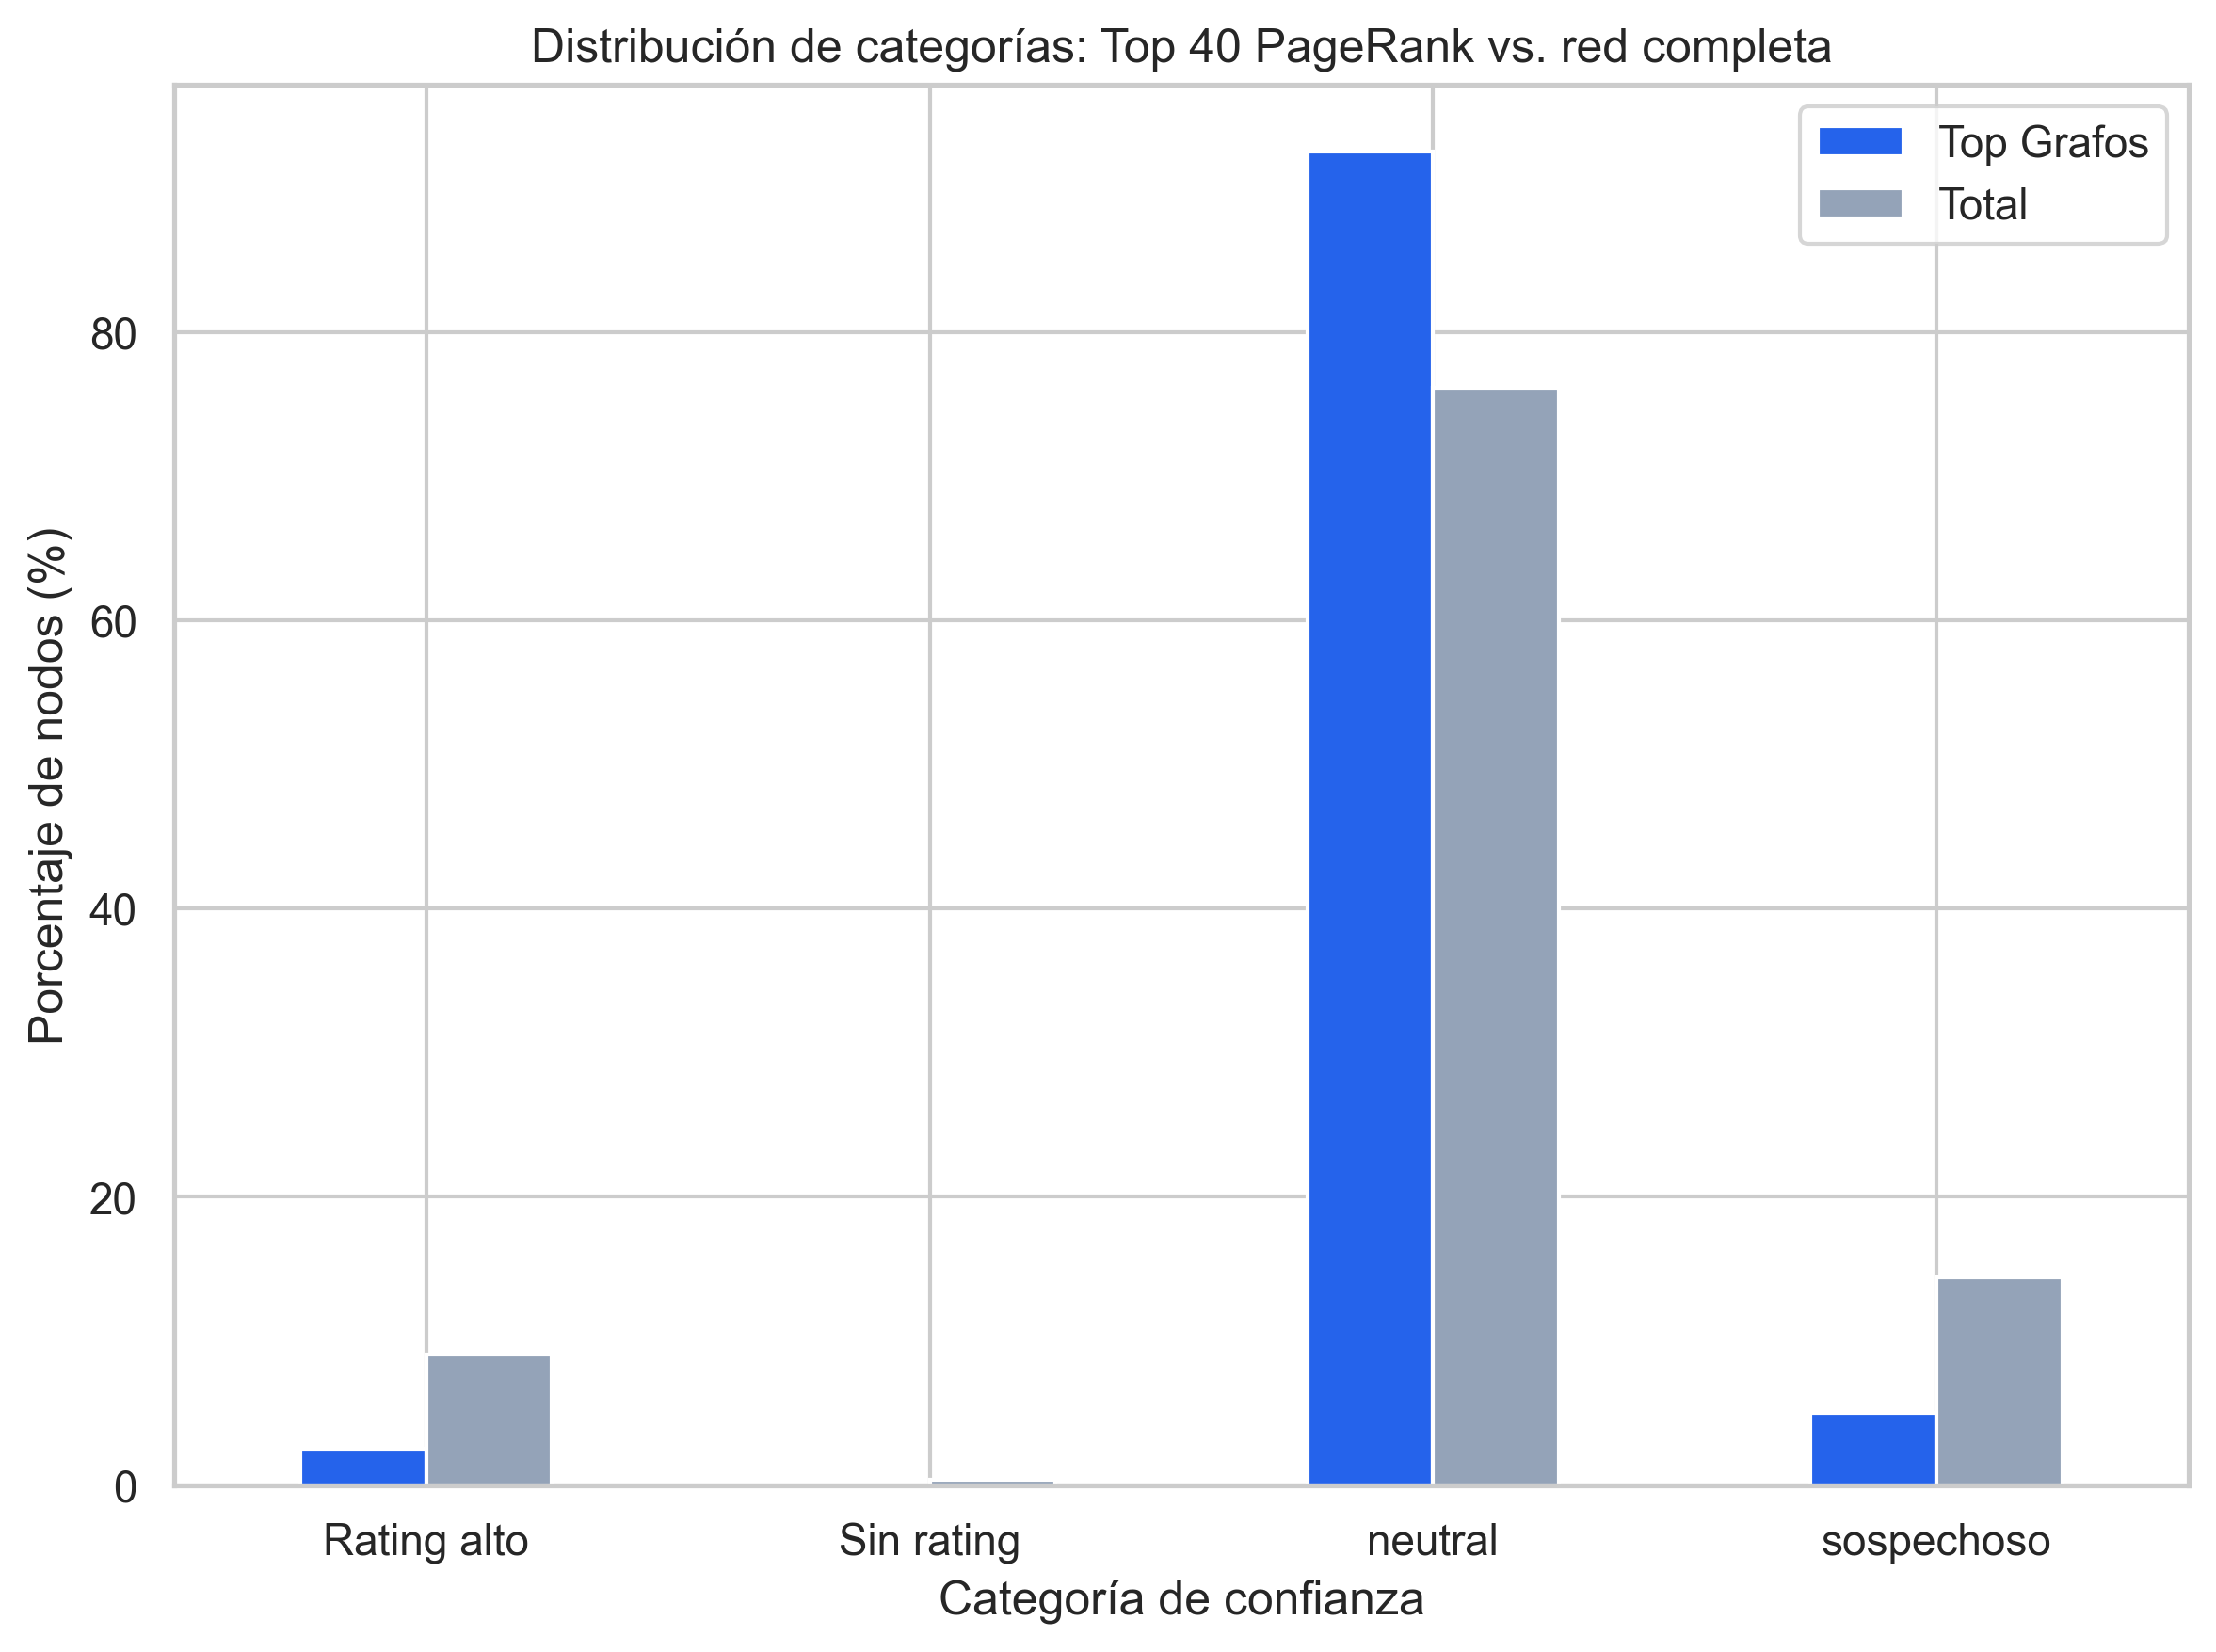
\includegraphics[width=0.8\textwidth]{plots/P7c_grafico_1.png}
\end{figure}


\begin{figure}[H]
\centering
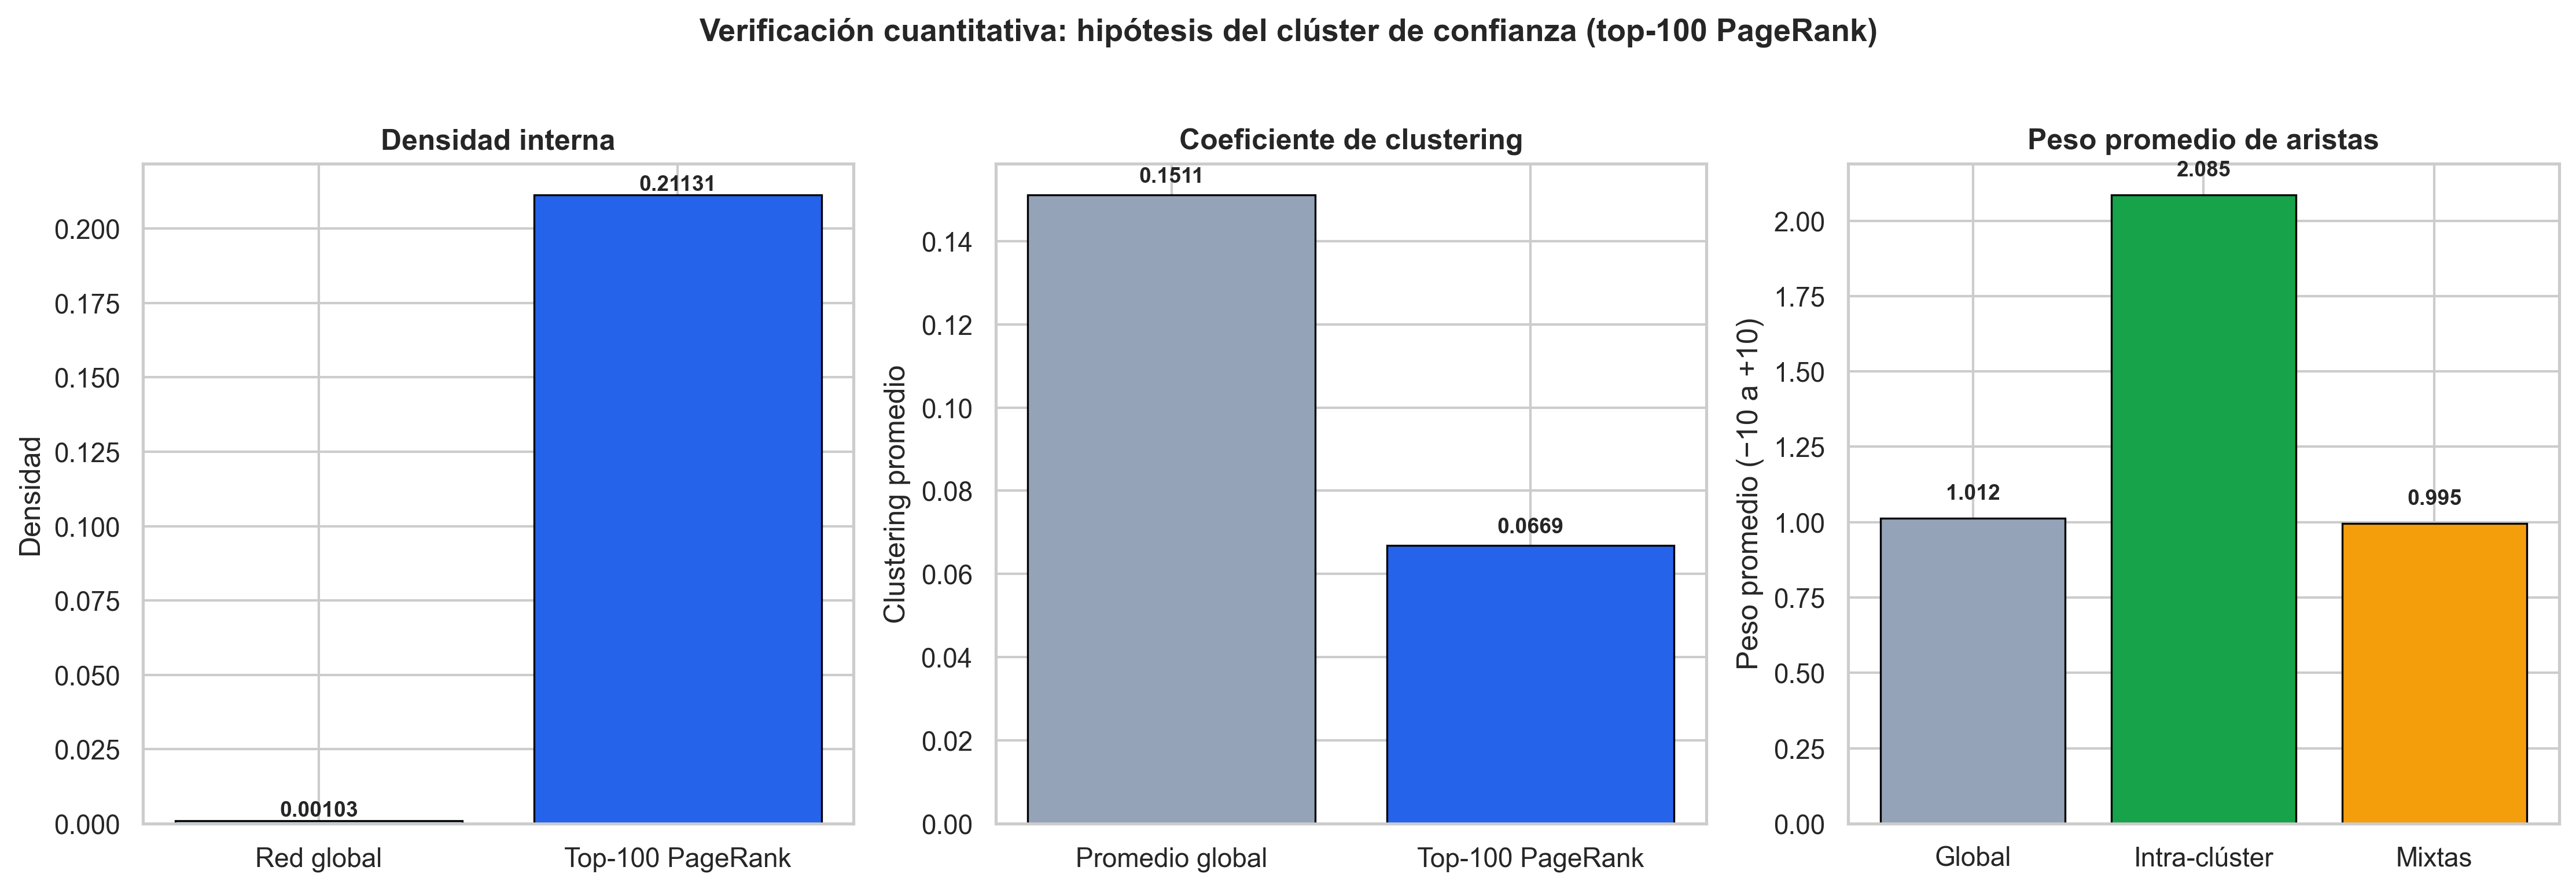
\includegraphics[width=0.8\textwidth]{plots/P7c_grafico_2.png}
\end{figure}


\textbf{Interpretacion}

El gráfico de distribución de categorías muestra una diferencia clara entre el top 40 PageRank y la red completa. Mientras que en la red global los nodos se distribuyen entre un rating alto, neutral y sospechoso. El top global está dominado casi en su totalidad por nodos de categoría neutral y rating alto, con los nodos sospechosos prácticamente ausentes, esto confirma que nuestra PageRank no está seleccionando nodos al azar, ni por volumen, sino que está filtrando hacia los grupos con reputaciones consolidadas

Las tres predicciones mencionadas anteriormente en nuestra hipótesis se confirmaron:

\textbf{Predicción 1 -- Densidad:} La densidad interna del top 100 PageRank supera con creces la densidad global de la red (0.001029). El factor de enriquecimiento obtenido indica que estos nodos están conectados entre sí de forma densa, por sobre el azar, funcionando como evidencia directa de que forman una comunidad cohesionada y no un conjunto disperso de usuarios populares independientes.

\textbf{Predicción 2 -- Clustering:} El coeficiente de clustering del top 100 (0.0669) resultó menor que el promedio global (0.1511), esto contradice nuestra predicción, sin embargo se puede explicar por qué nodos de un alto grado como el nodo 24 pueden tender a que, al estar conectado con cientos de nodos , sea poco probable que todos sus vecinos también se conecten entre sí , luego aunque la red en su alrededor sea densa, se tiene que la densidad del clúster local no es un indicador adecuado.

\textbf{Prediccion 3 -- Homofilia de confianza:} El peso promedio de las aristas dentro del clúster(2.085) es notablemente mayor que el de las aristas mixtas (0.995) y que el global (1.012). significando así que cuando dos nodos del núcleo se califican , lo suelen hacer con el doble de rating positivo que el promedio de la red, de forma aproximada, es decirla con fianza no es solo estructural sino que cualitativa, de forma que los miembros se valoran más alto entre ellos

En total 2 de las 3 predicciones se confirmaron, y la que no se cumplió tiene una explicación coherente con la presencia de un hub , de forma que nuestra hipótesis de que la PageRank identifica un núcleo de confianza densamente Interconectado y con rating positivos queda respaldada.



\subsection*{P8: Discusión, limitaciones y conclusiones}

\textbf{Contraste con la hipotesis inicial}

Nuestra hipótesis planteaba que los usuarios con un mayor page rank formarían un clúster de confianza densamente interconectado con 3 predicciones concretas:
- Mayor densidad interna
- Mayor coeficiente de clustering local
- peso promedios más positivos dentro de este clúster

Dos de las tres predicciones se confirmaron, y una no lo hizo, la densidad interna del top-100(0.2113) supera con creces a la densidad global (0.001029) y las aristas intra-cluster también poseen un promedio de pesos de 2.085 en relación con las 0.995 de las aristas mixtas sin embargo los coeficientes de clusterring local del top 100 resulto ser inferior al promedio global, cosa que contradice nuestra segunda predicción, esto no necesariamente invalida la hipótesis, sin embargo da a entender que se posee una presencia de "hubs" donde los nodos presentan una alta conexión con un nodo específico, luego los nodos con una cantidad de conexiones altas presentan que en relación con sus vecinos se tiene una interconectividad relativamente baja por la improbabilidad de que todos los vecinos estén conectados entre sí.

\textbf{¿La pregunta quedó respondida?}
La pregunta era: ¿Existe dentro de la red Bitcoin OTC un clúster nuclear de usuarios con altos ratings positivos entre sí, y puede el PageRank identificar a sus miembros más centrales?

Si, En ambas partes. El clúster existe con propiedades medibles. Densidades aproximadamente 200 veces mayores a las globales, y rating intra-cluster el doble de positivos que el promedio, el análisis de las categorías confirman que los nodos sospechas son ausentes del Top PageRank mientras que están presentes en la red general, Las pagerank Discriminan activamente haciendo que se tenga un núcleo de confianza en la plataforma

\textbf{Limitaciones del método y los datos:}

El modelo de marcha aleatoria ignora el signo de las aristas, una calificación de -10 posee el mismo peso que una de 10 en el momento de la Construcción de $H$ - que la hipótesis se haya confirmado indica que esta red de nodos centrares acumulan predominantemente calificaciones positivas, pero eso no es garantizado por el método, el filtro de rating\_prom\_recibidos de P7(a) es únicamente un parche para poder ayudarnos con el momento de hacer los análisis.


\textbf{Preguntas nuevas que surgieron del análisis}

¿Cómo se podría cambiar el clúster si se usa un PageRank ponderado, donde el peso de transición es proporcional a los ratings? ¿Quiénes subirían y bajarían respecto a nuestro análisis actual?

¿Se puede crear un clúster análogo a este pero de desconfianzas? Es decir, un PageRank sobre aristas negativas, de forma que podamos identificar los nodos que presentan más denuncias

\textbf{Resultados principales}

En un mercado donde nadie se conoce de antemano y se mantiene un anonimato, los traders más confiables parecen juntarse y encontrándose, calificándose entre ellos de forma positiva, haciendo y formando un cluster , o gremio de traderas con una alta reputación, en ese sentido el algoritmo de PageRank identifico a los miembros centrales de este gremio, los más respaldados por personas respaldadas, obteniendo de esa forma que este gremio existe y que posee una forma clara, sus miembros se conectan entre si con una densidad varias veces mayor a la del resto de los traders, y cuando se califican entre si, lo hacen con el doble de positiva en relación con el promedio.





\end{document}